\documentclass[11pt]{report}
\newcommand{\userName}{Rebecca Miko}
\newcommand{\institution}{University of Hertfordshire}

%Packages
\usepackage{graphicx}
\usepackage{xr}
\usepackage{hyperref}
\usepackage{geometry}

\geometry{margin=1in}



% Begin document
\begin{document}

\pagenumbering{arabic}
\begin{center}
{\Huge Progress Report}
\end{center}
\section*{Abstract}
The olfactory bulb in mammals is responsible for receiving, processing and relaying olfactory information (odours). This project investigates how naturalistic temporally fluctuating odour signals are processed and which neurons 
or neural mechanisms are able to extract information from these signals. Multiple computation models were created to represent different OB circuits between periglomerular cells and mitral cells using NEURON (Hines and Carnevale, 2006, 2001). 
The results show that the strength and frequency of these odour signals can be determined by looking at a combination of the latency and the firing rates of the output from the mitral cells. 

\section*{Research question:}
Can we predict the strength and frequency of the input by looking at two features: Firing Rates and Latency?\\

First, we look at 3 input frequencies (1,10 and 40\,Hz) and 2 input strengths (0.315 and 0.54\,nA):
\begin{figure}[!ht]
\centering
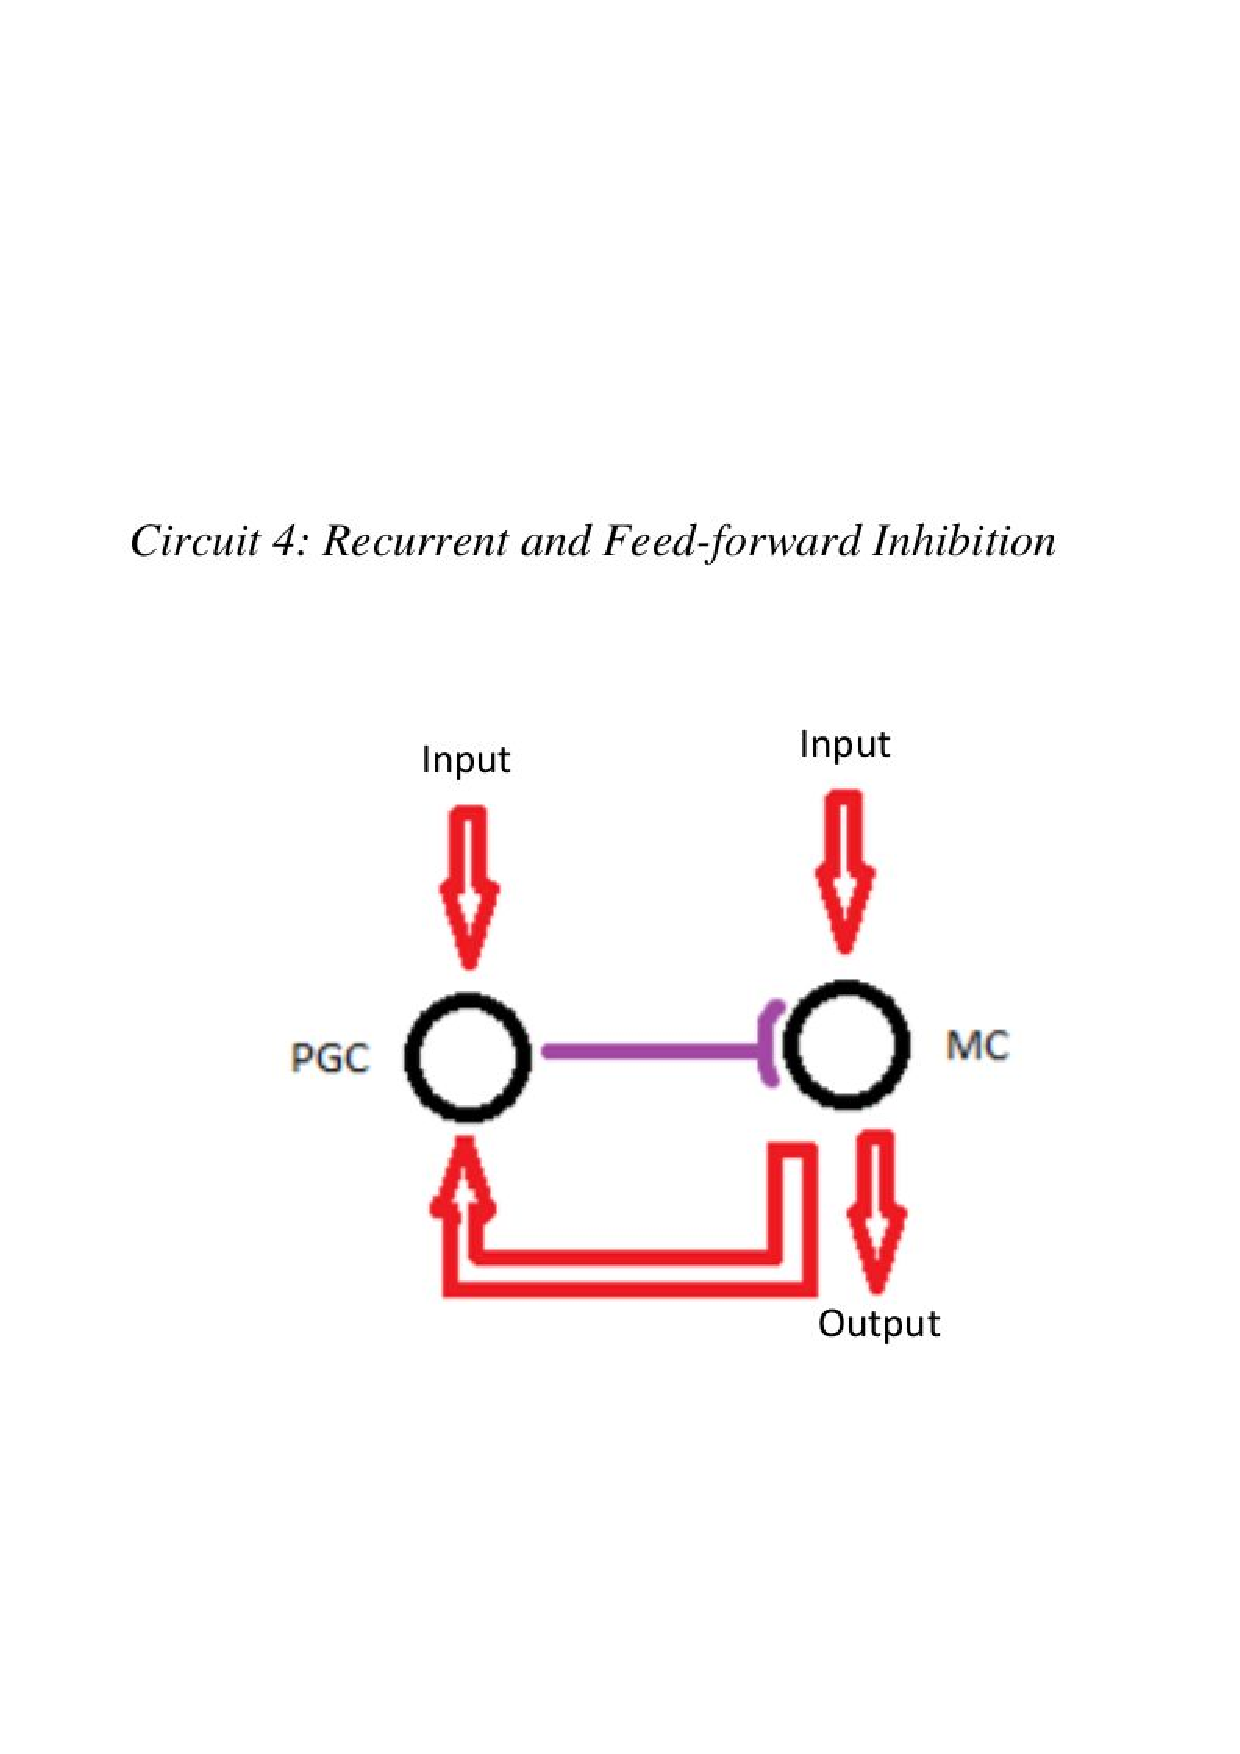
\includegraphics[trim={0 6cm 0 8cm},clip, scale=0.5]{Analysis-6-11-17/Circuit_4.pdf}
\caption{The full model.}
\end{figure} 

Figure 1 shows the full model (denoted as circuit 4). The PGC (periglomerular cell) and the MC (mitral cell) both recieve input, both the feed-forward and recurrent inhibition is considered, and the output from the MC is analysed. 
\newpage

\begin{figure}[!ht]
\centering
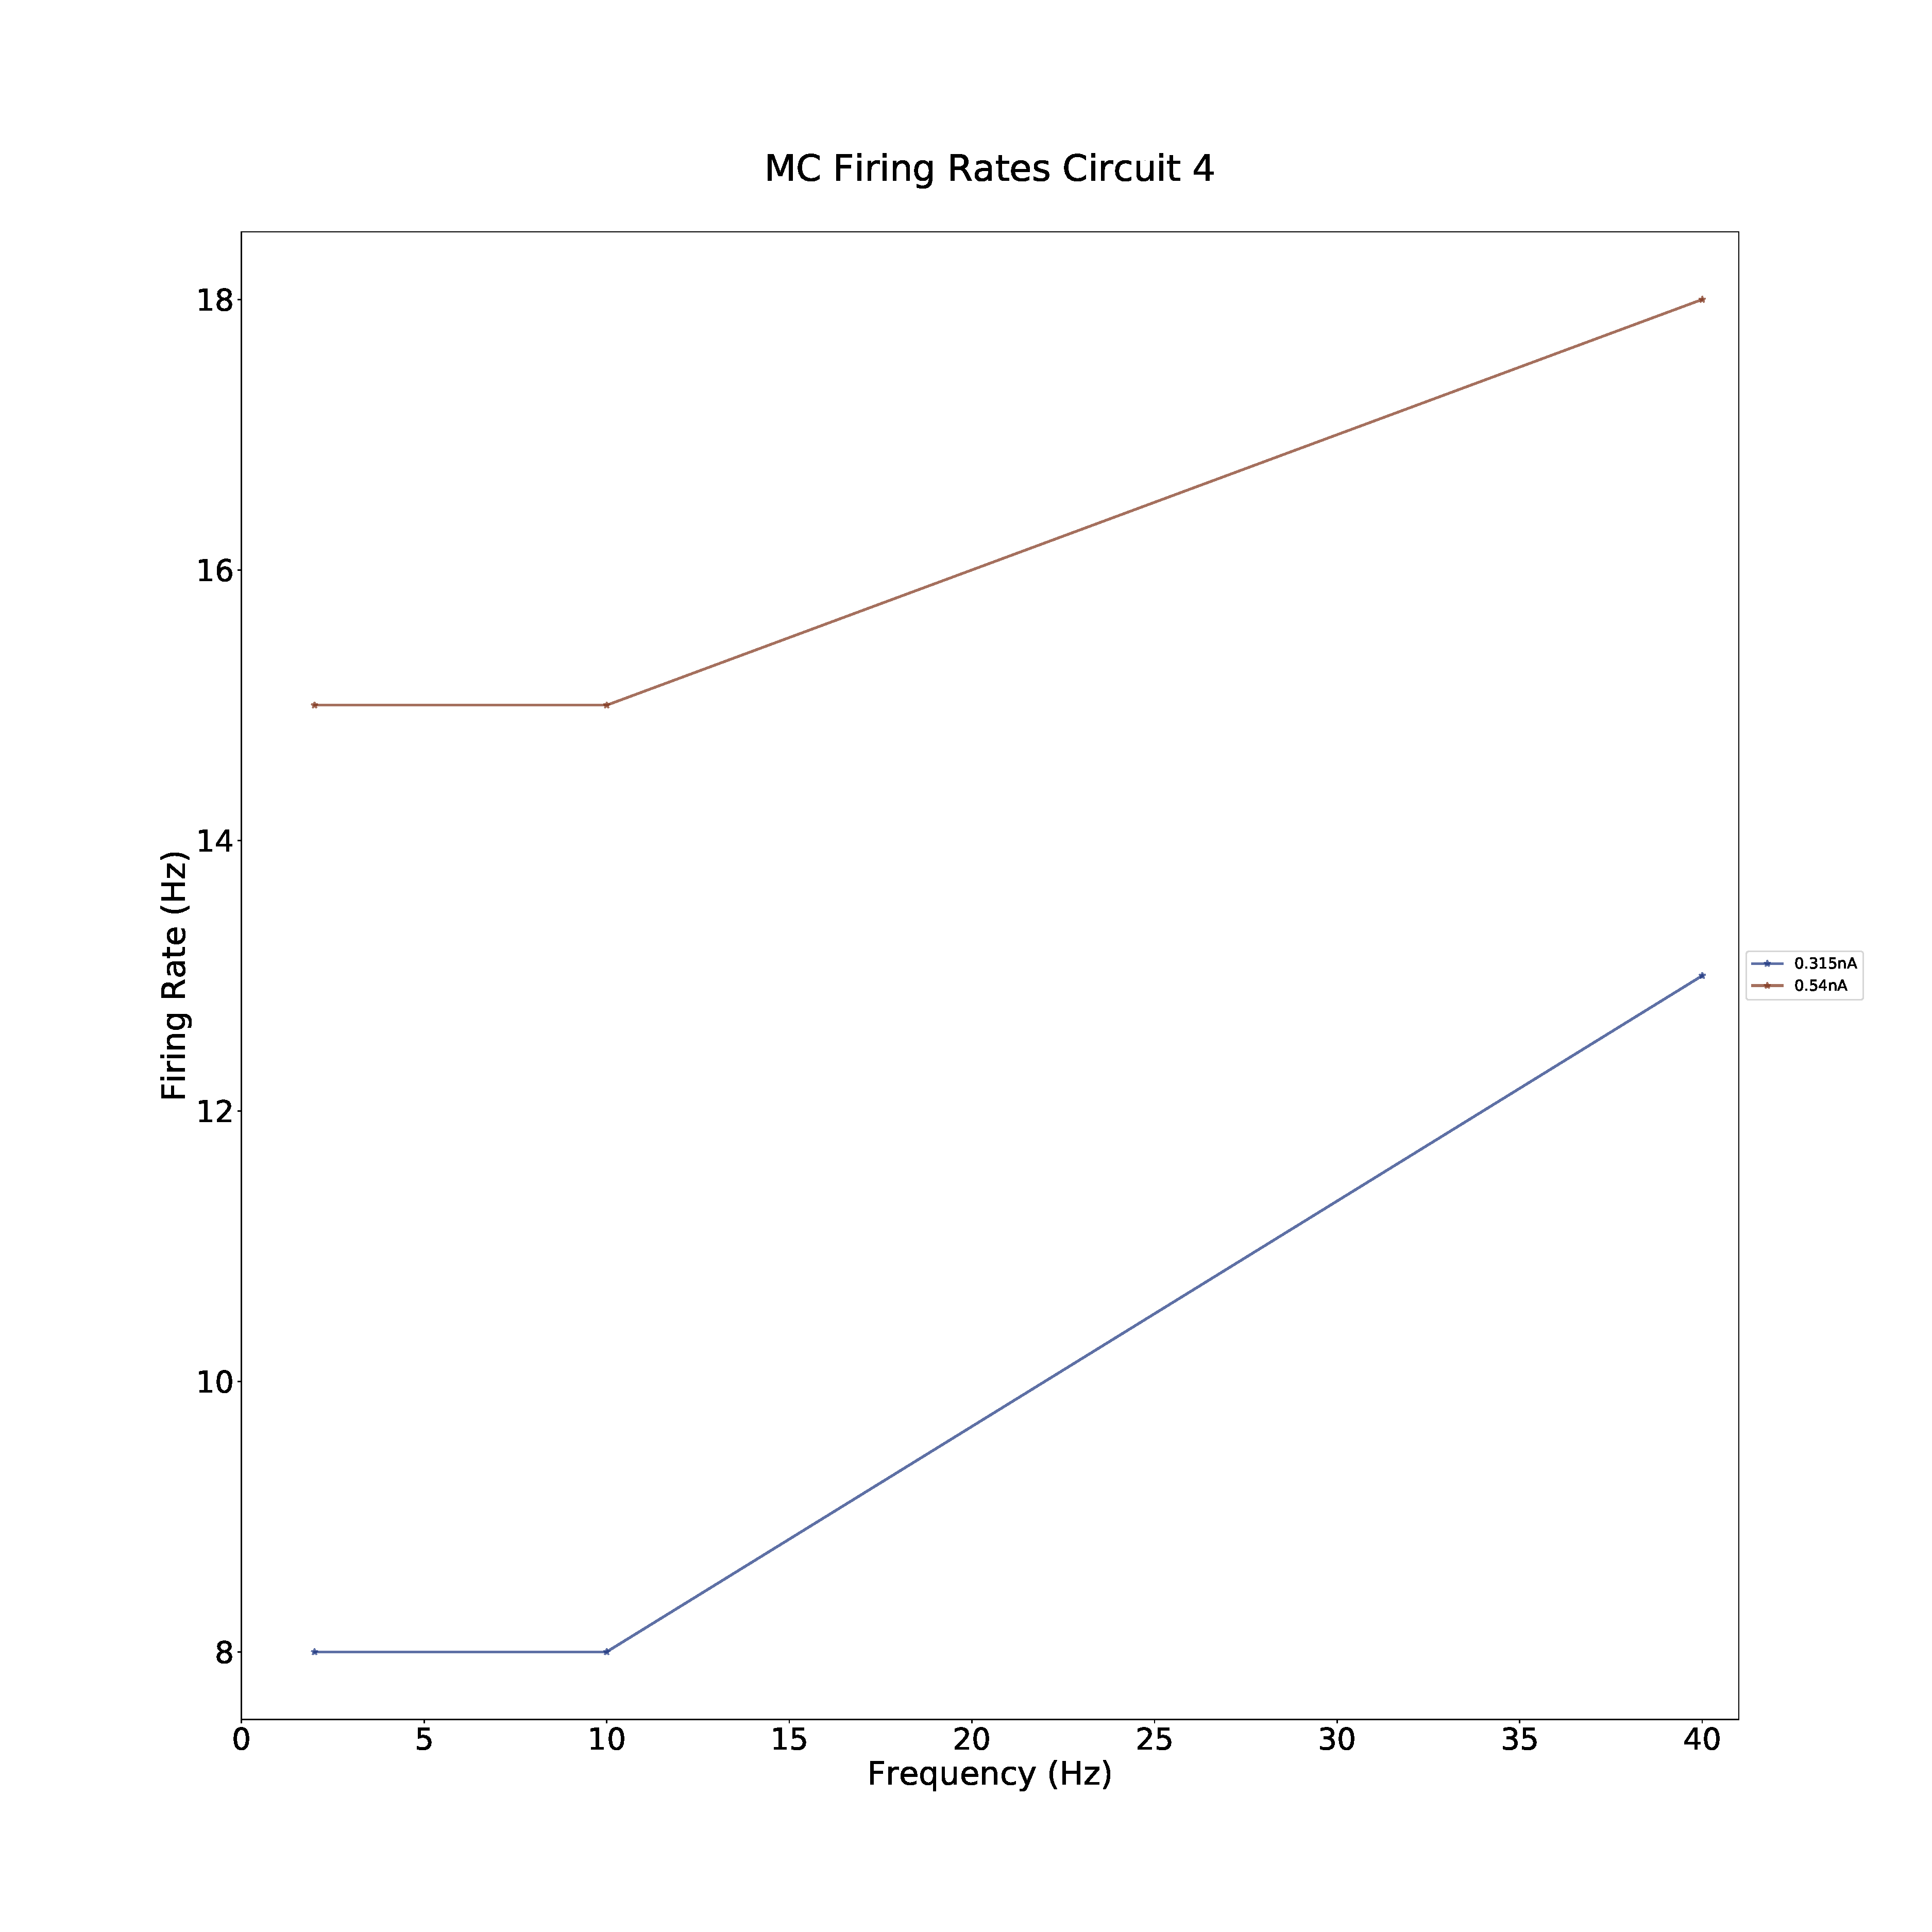
\includegraphics[scale=0.3]{Analysis-6-11-17/MC_firing_rate_C4.pdf}
\caption{The mitral cell firing rates for circuit 4.}
\end{figure} 

In figure 2, it is clear that the firing rates can be used to determine the strength of the input current. However, the frequency of the input current is still unclear. 
\newpage

\begin{figure}[!ht]
\centering
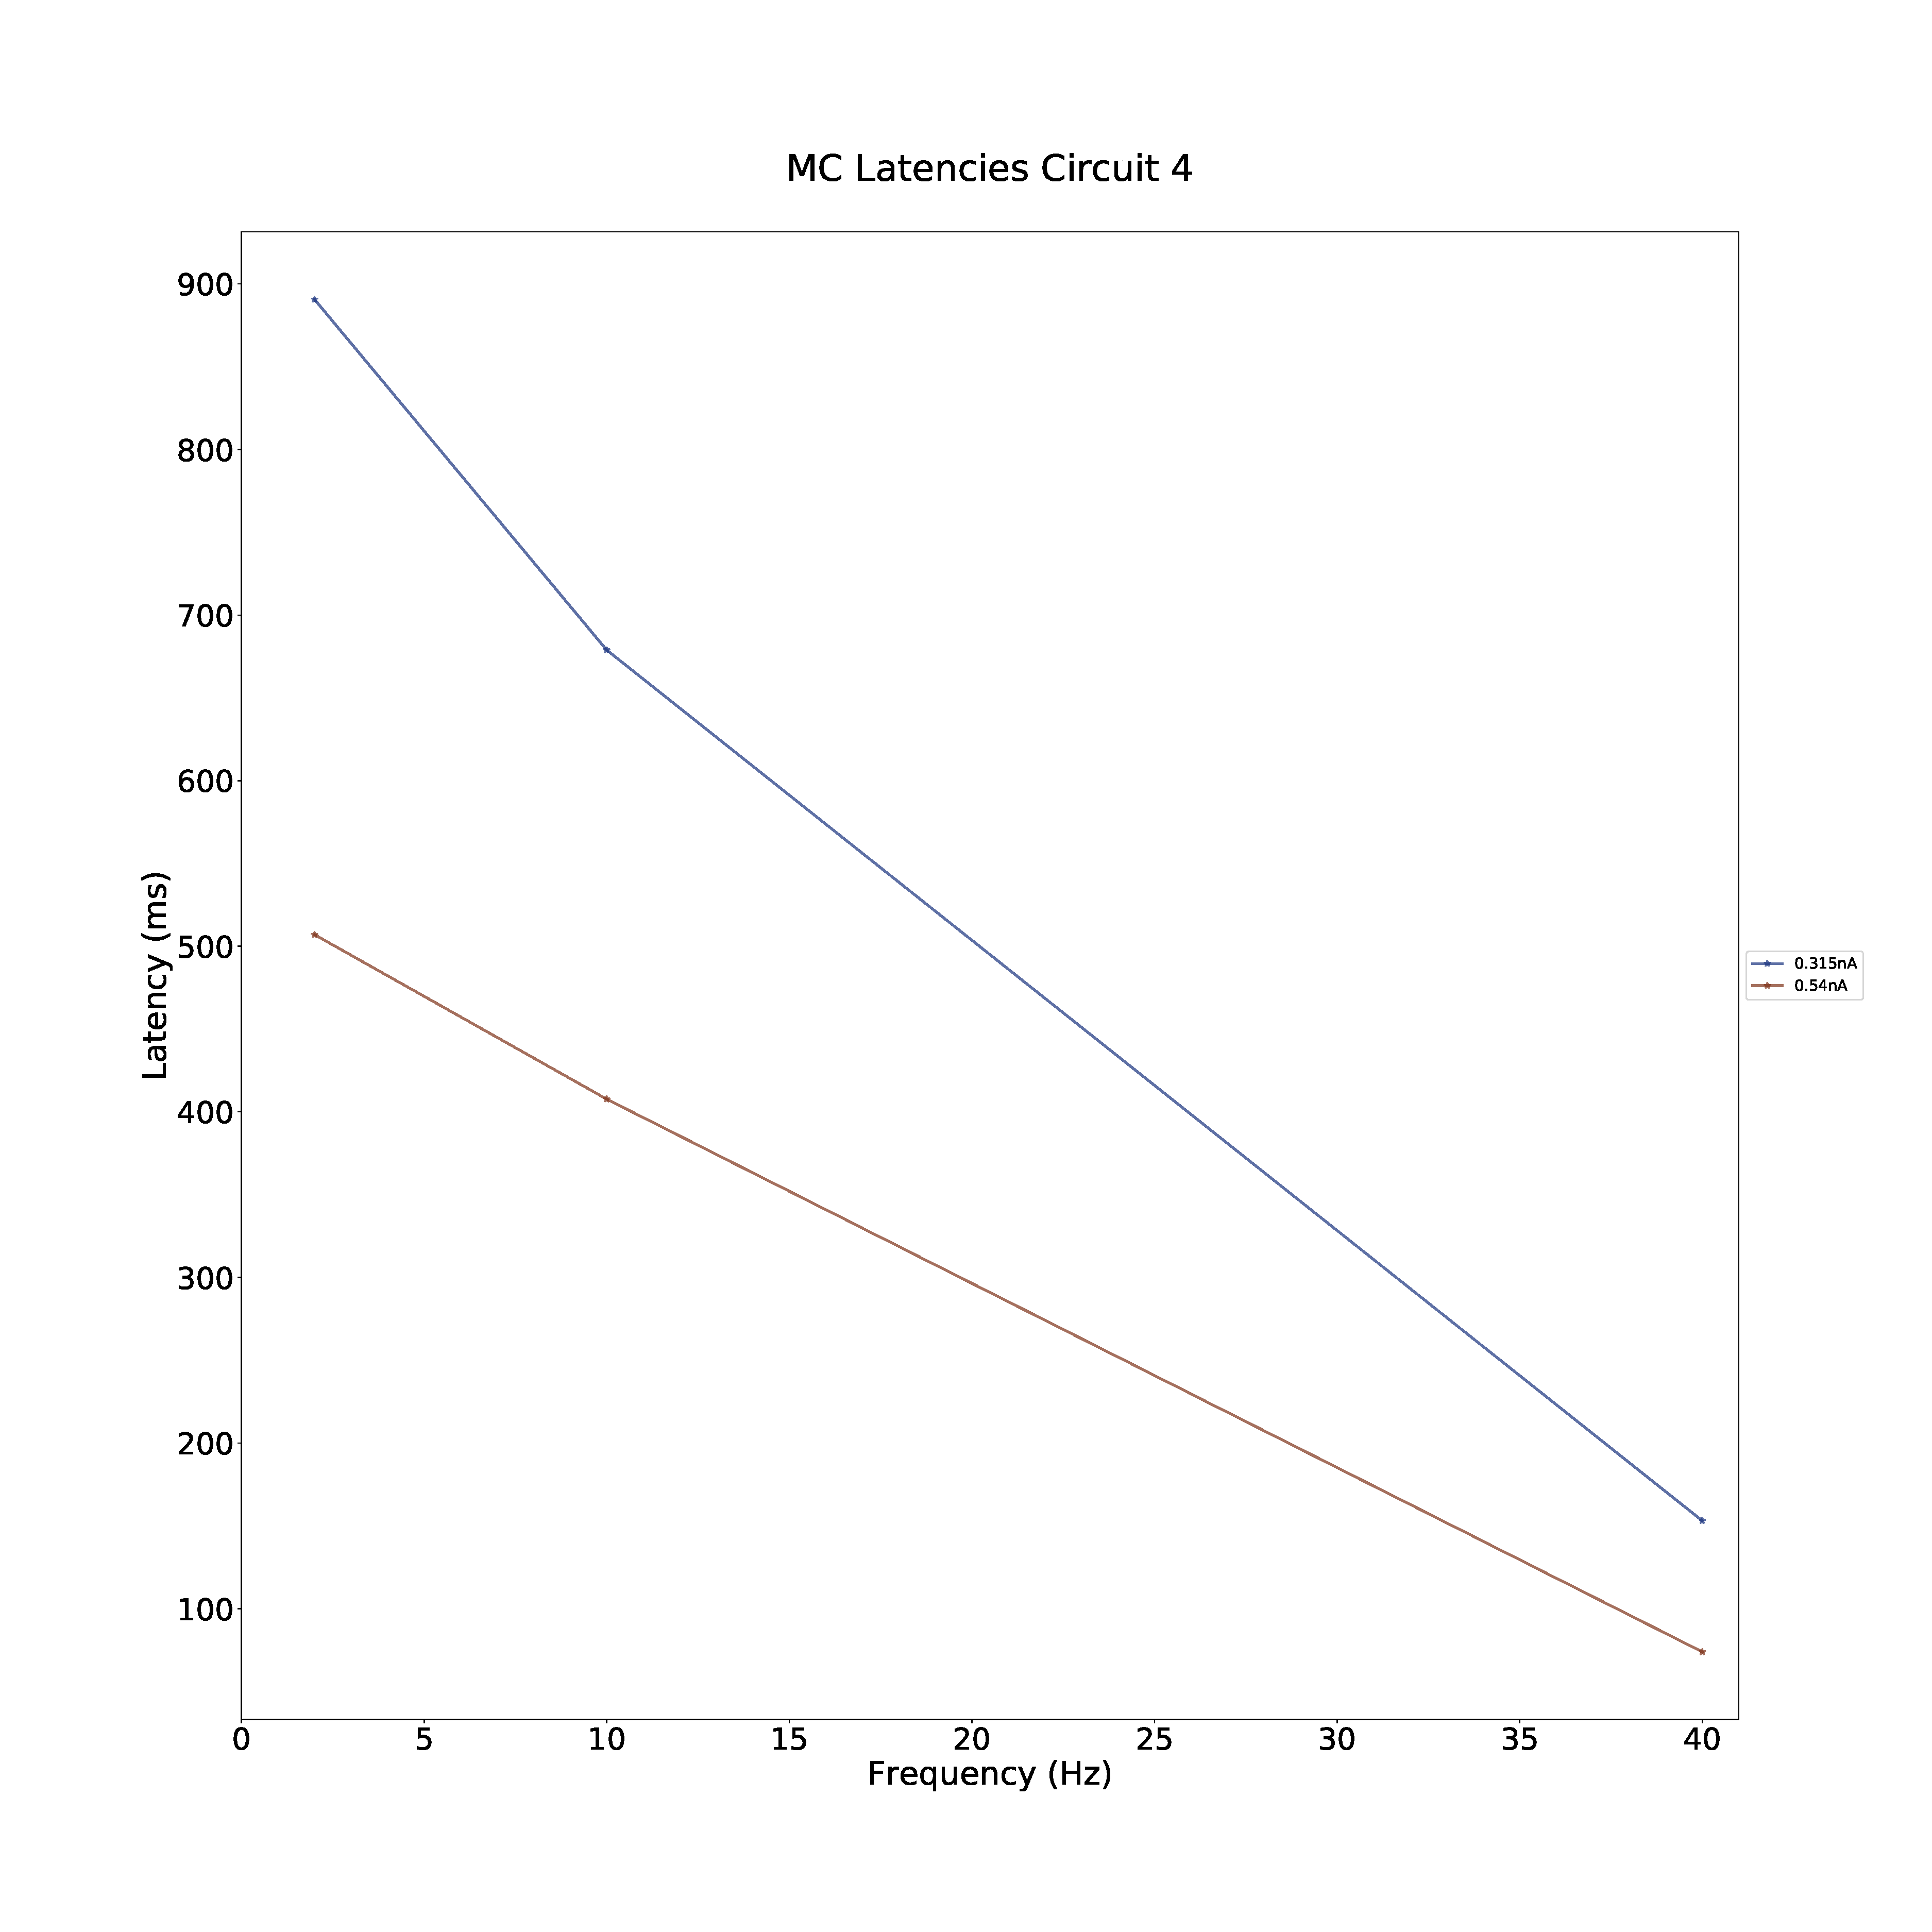
\includegraphics[scale=0.3]{Analysis-6-11-17/MC_latencies_C4.pdf}
\caption{The mitral cell latencies for circuit 4.}
\end{figure} 

Figure 3 shows that we can determine the frequency of the input from the latencies, if we know the strength of the input. Therefore, we can predict the strength and frequency of the input by looking at a combination of both firing rates and latency.

\paragraph{Underlying Mechanisms}
The strength and frequency of the input can be predicted by looking at the firing rates and latency, as described above. What mechanism is responsible for these results?

\begin{figure}[!ht]
\centering
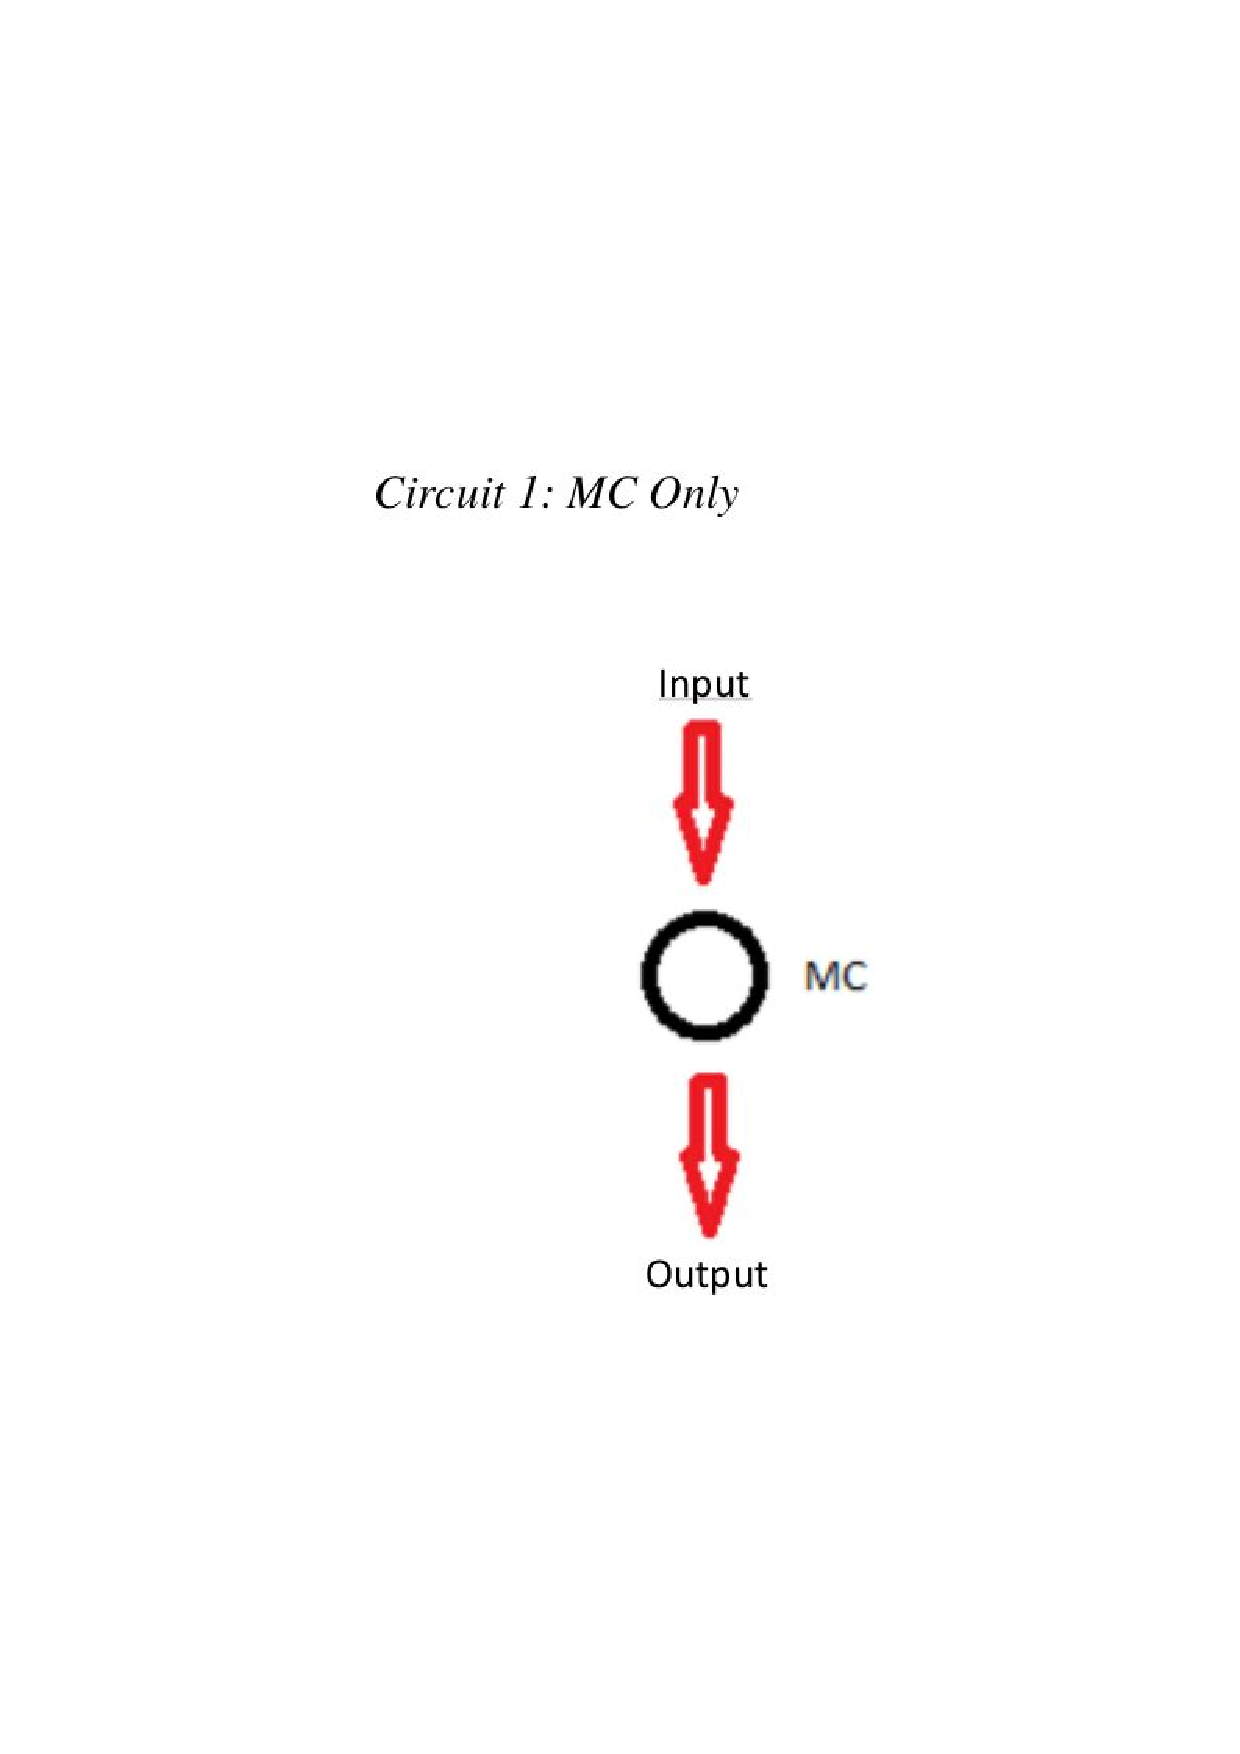
\includegraphics[trim={0 6cm 0 8cm},clip, scale=0.5]{Analysis-6-11-17/Circuit_1.pdf}
\caption{Circuit 1. This focuses on the mitral cell only.}
\end{figure} 

\begin{figure}[!h]
\centering
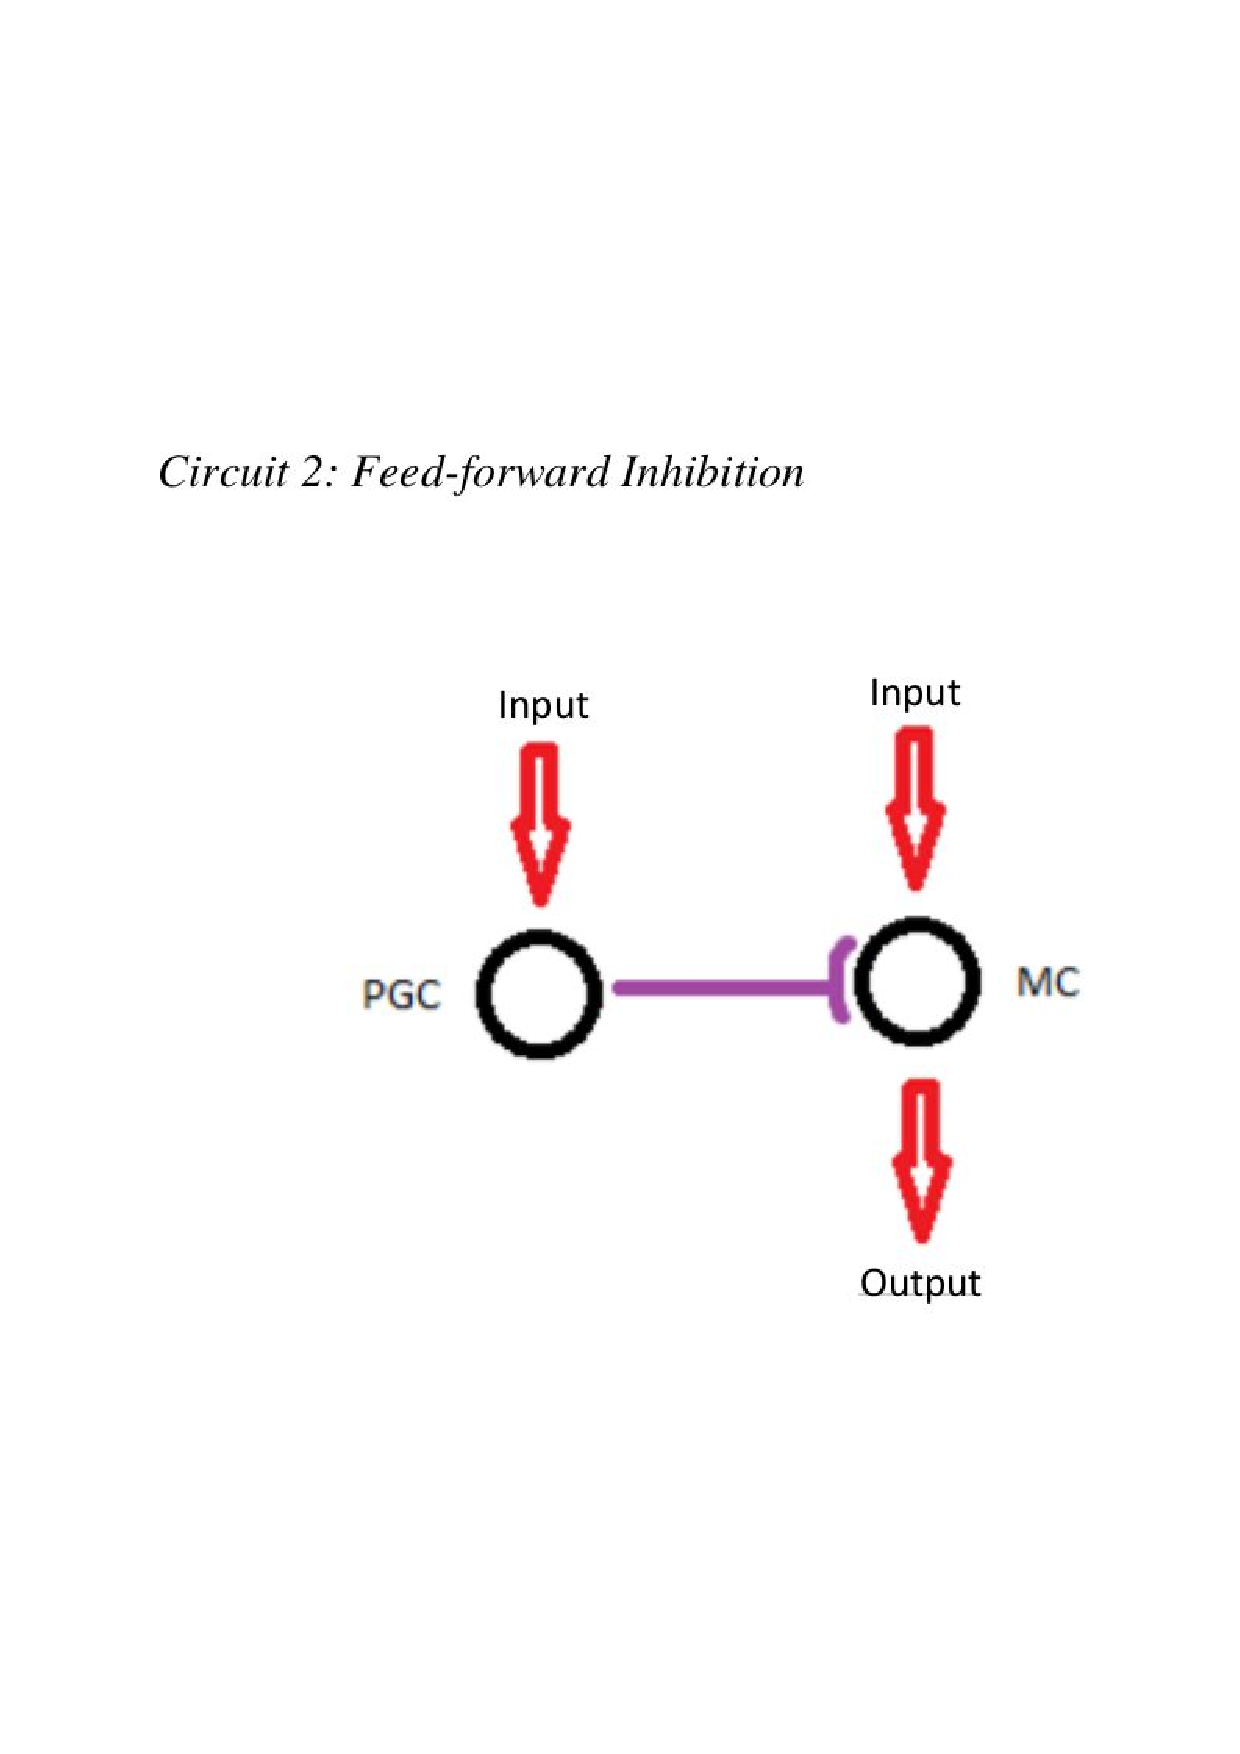
\includegraphics[trim={0 6cm 0 6cm},clip, scale=0.5]{Analysis-6-11-17/Circuit_2.pdf}
\caption{Circuit 2. This focuses on the feed-forward inhibition.}
\end{figure} 
\newpage

\begin{figure}[!ht]
\centering
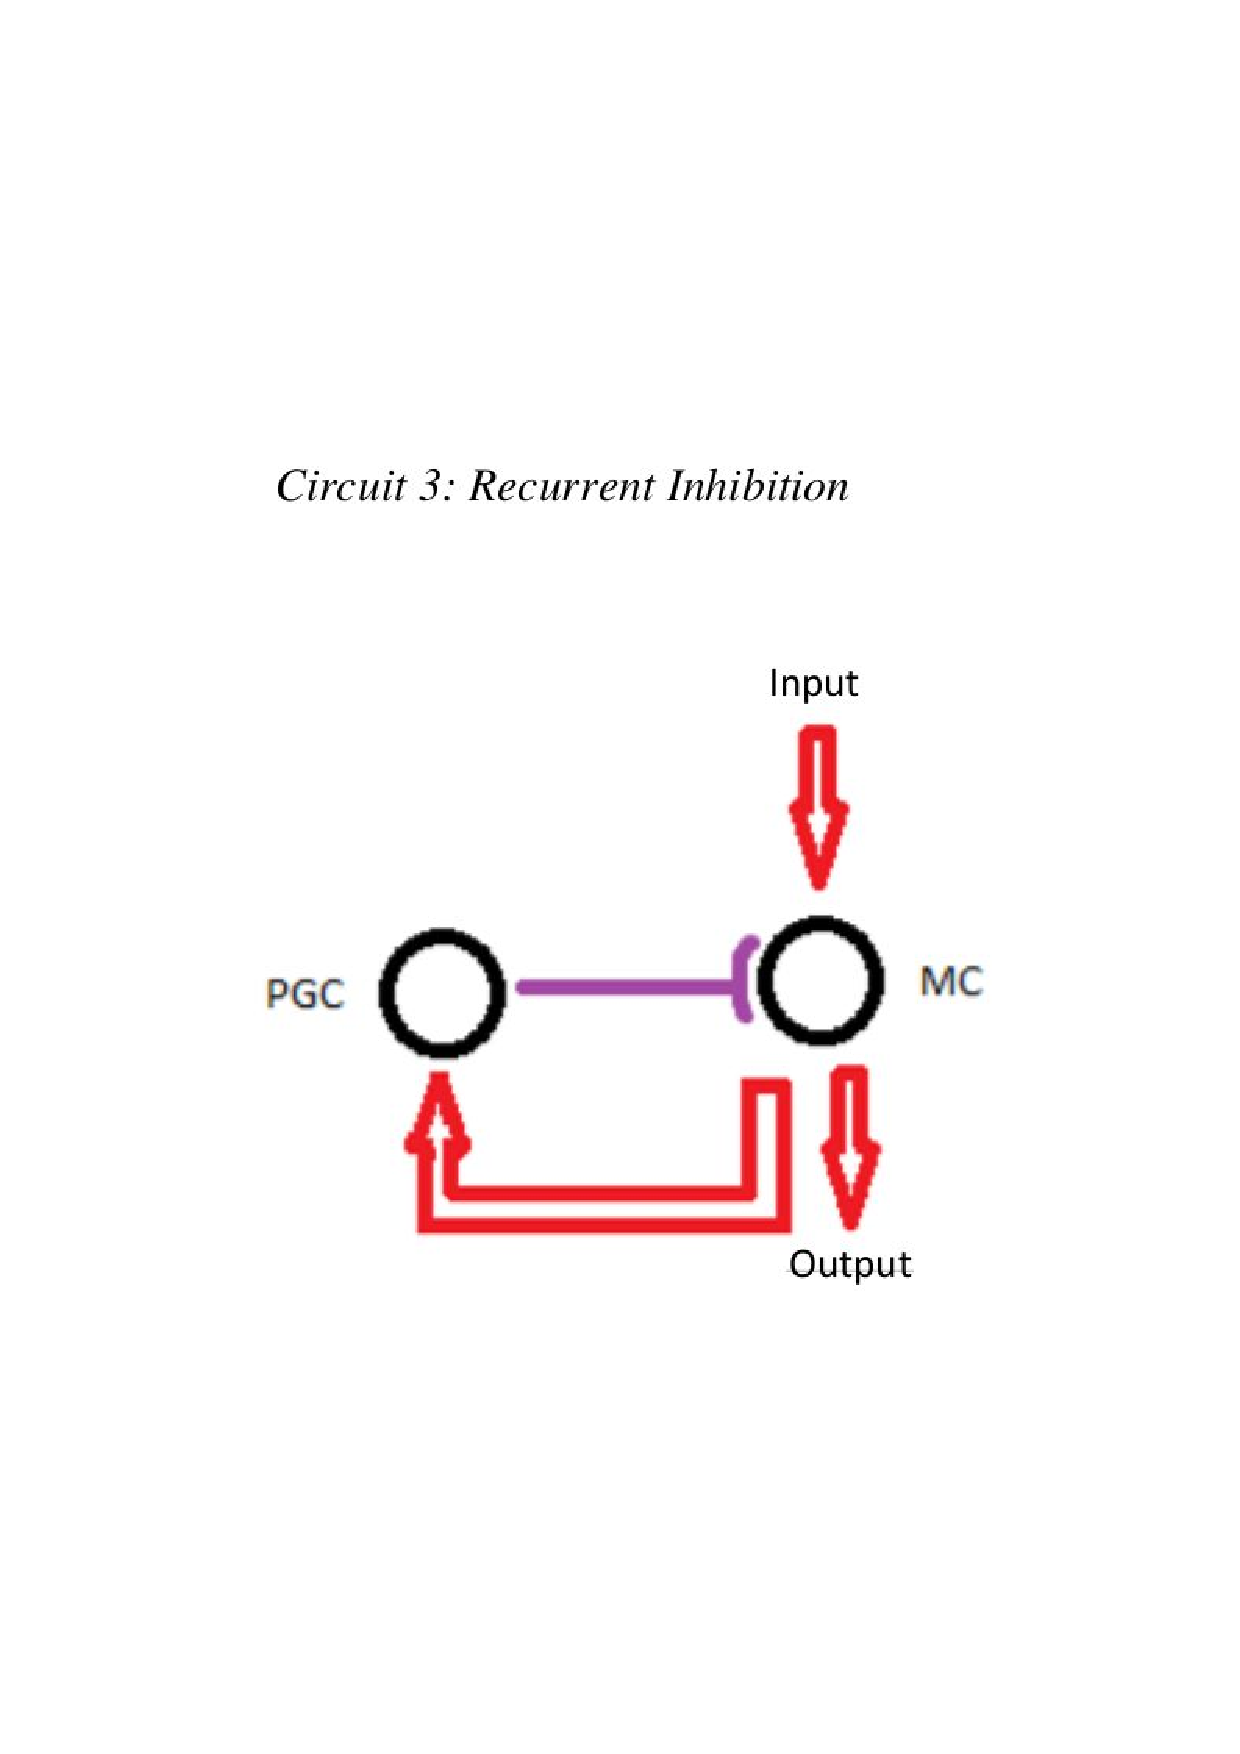
\includegraphics[trim={0 6cm 0 6cm},clip, scale=0.5]{Analysis-6-11-17/Circuit_3.pdf}
\caption{showing circuit 3. This focuses on the recurrent inhibition.}
\end{figure} 

Each aspect of the model was analysed individually, see figures 4, 5 and 6. Therefore, we can determine which mechanism is responsible for results found in figures 2 and 3.
\newpage

\begin{figure}[!ht]
\centering
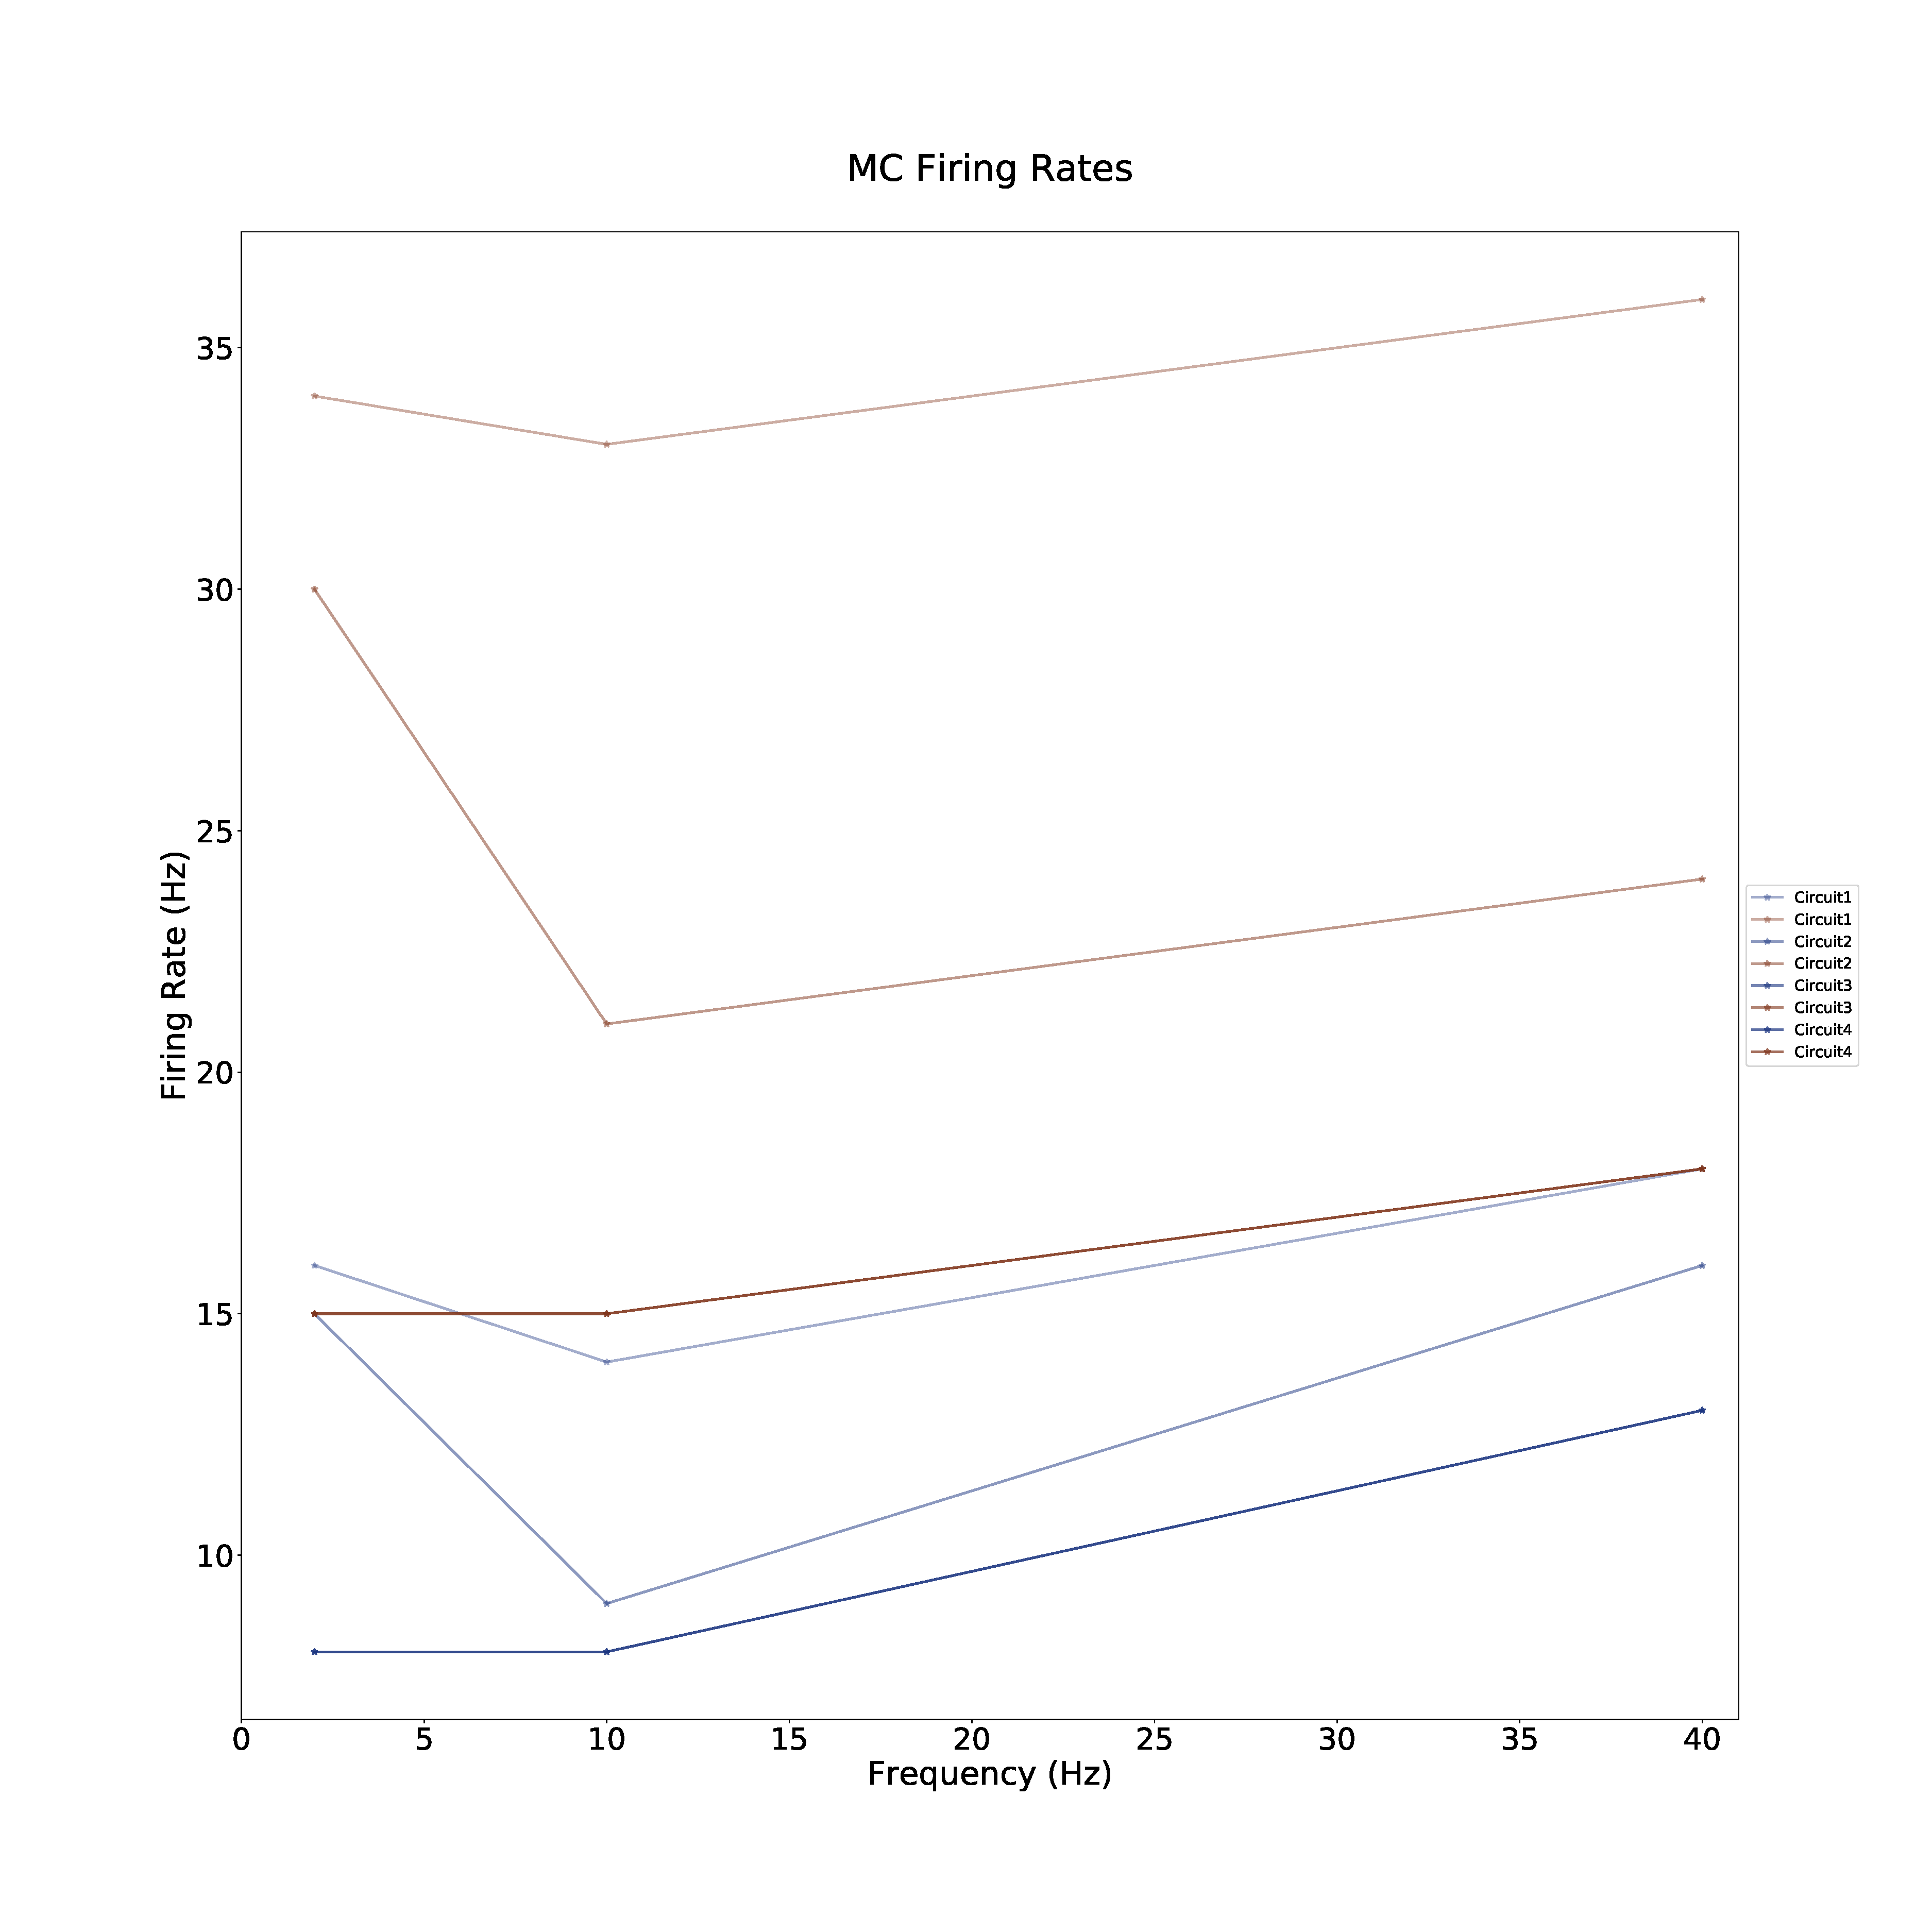
\includegraphics[scale=0.3]{Analysis-6-11-17/MC_firing_rate.pdf}
\caption{showing the mitral cell firing rates for all circuits.}
\end{figure} 

\begin{figure}[!ht]
\centering
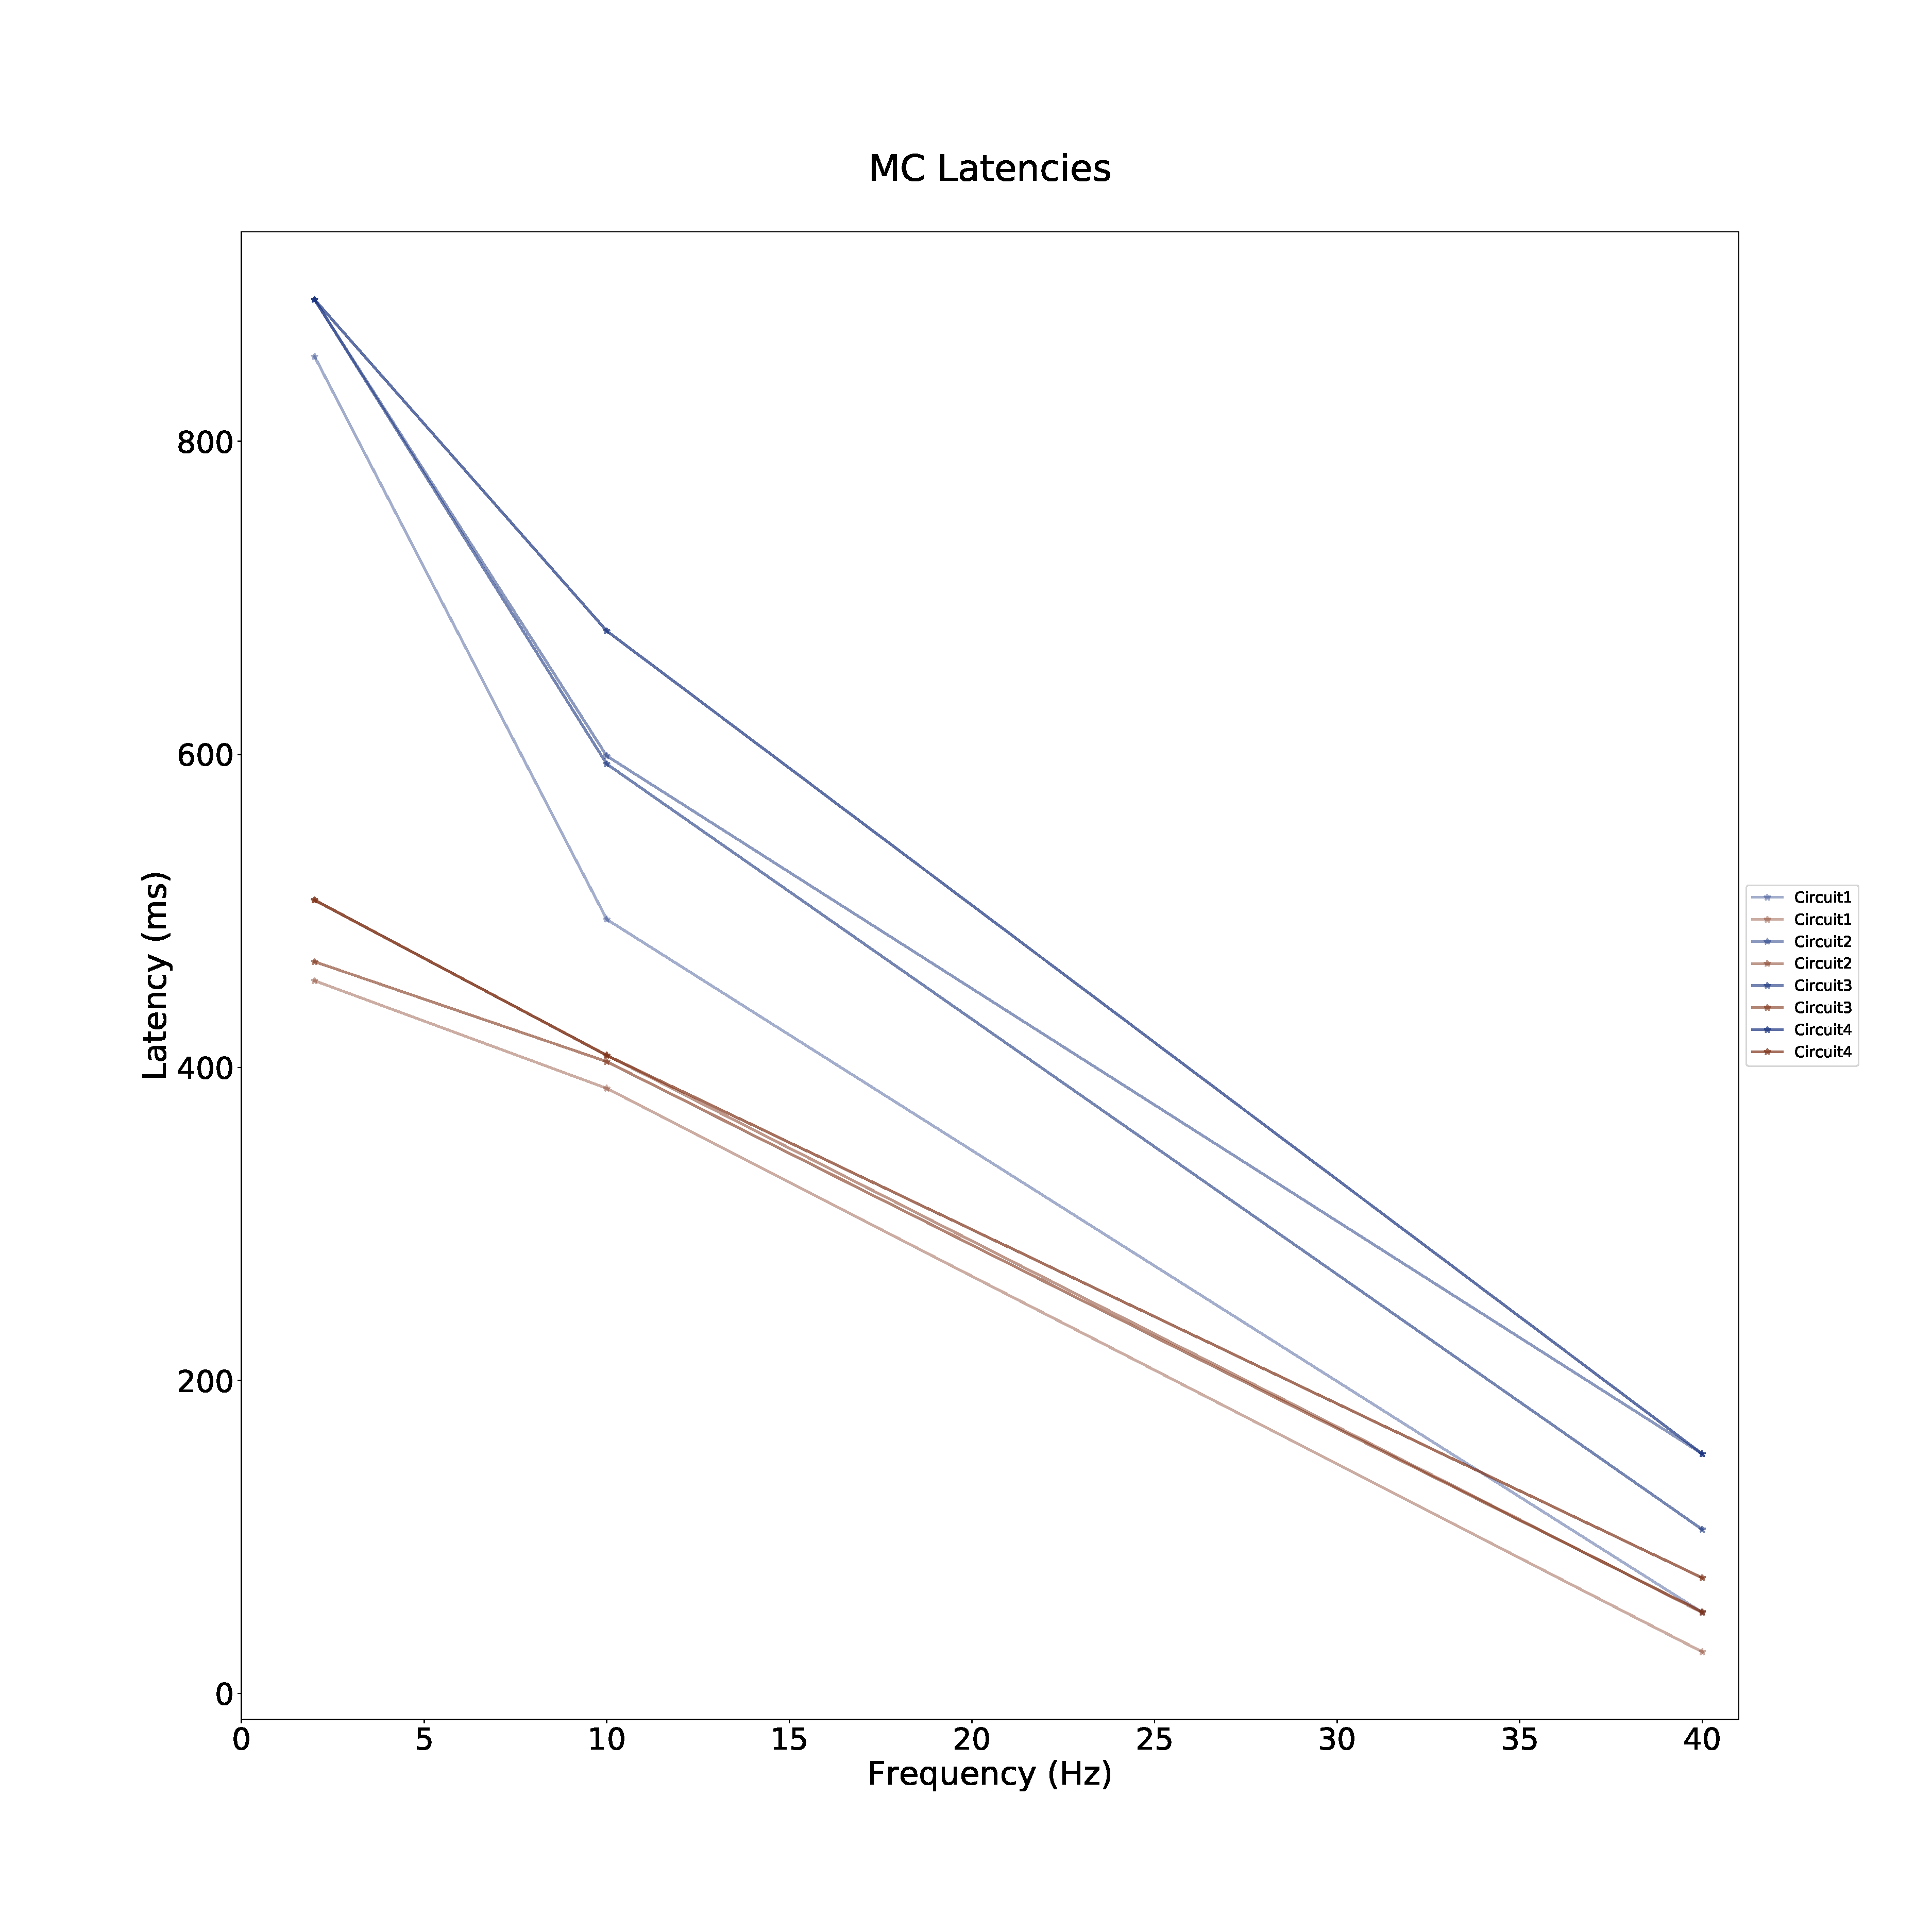
\includegraphics[scale=0.3]{Analysis-6-11-17/MC_latencies.pdf}
\caption{showing the mitral cell latencies for all circuits.}
\end{figure}

We see that the 'frequency-independence' of the firing rates as well as the inverse proportionality of input frequency and latency already holds for the MC only circuit (circuit 1). Therefore,
for these very simplistic inputs, the intrinsic mechanisms of the mitral cells are enough and none of the inhibitory circuits is needed.

\section*{Predictor}
Next, we want to look at the prediction of input strength and frequency in a more quantitative way. To this end, we simulated 49 different combinations of
strength and frequency (7 strengths: ... ; and 7 frequencies: 1,2,5,10,20,30 and 40\,Hz) and extracted the mean firing rate and the latencies from the MC responses.

If we plot firing rate against frequency \ref{fig:frate-freq}, we can see that the firing rate is almost independent from the input frequency.

\begin{figure}[!ht]
\centering
\includegraphics[scale=0.3]{}
\caption{Firing rate vs input frequency plot.}
\label{fig;frate-freq}
\end{figure}

Furthermore, if we plot latency versus input strength \ref{fig:lat-strength}, we can also see that the latency seems only to depend on the frequency and not on the strength.

Thus, as the first and simplest predictor, we use two linear functions that relate input strength to firing rate and input frequency to latency, respectively. Fitting the two functions to our data,
gives us:
\[
 FR(s) = 32.26\cdot s - 0.59
\]

and 

\[
 L(f) = -16\cdot f + 645.4
\]

As a first test of the predictor, we predict the firing rate (FR) and the latency (L), for two pairs of input strength and frequency: (0.5\,nA,13\,Hz) and (0.3\,nA,1.7\,Hz).
As predictions we get: FR=15.5\,Hz and L=437.4\,ms in the first case and  FR=9.1\,Hz and L=618.2\,ms in the second.
The actual results from the simulations are: FR=13.5\,Hz and L=475.6\,ms and FR=7.7\,Hz and L=711.1\,ms, respectively.

Next, to get a more detailed test, we draw 25 new random pairings of strength (range:-) and frequency (range:0.5-50), predict firing rate and latency and compare them to the actual simulation results.
We calculated the root mean squared error (RMS) for firing rate and latency:

\[
 RMS(x^{pred},x^{act})=\sqrt { \sum_i (x^{pred}_i - x^{act}_i)^2}
\]




\end{document}